\documentclass[12pt,a4paper]{article}
\usepackage[utf8]{inputenc}
\usepackage[T1]{fontenc}
\usepackage[english]{babel} % English ist korrekt für eure Anforderungen
\usepackage{graphicx}
\graphicspath{{../assets/}{assets/}{images/}}
\usepackage{float}
\usepackage{amsmath}
\usepackage{hyperref}
\usepackage{booktabs}
\usepackage{caption}
\usepackage{setspace}
\usepackage{geometry}
\usepackage{titlesec}
\usepackage{fancyhdr}
\setlength{\headheight}{19pt}
\usepackage{csquotes}
\usepackage[nottoc]{tocbibind}
\usepackage{xcolor}

% Bibliography Settings
\usepackage[style=authoryear, backend=biber, maxcitenames=2, maxbibnames=99, uniquelist=false]{biblatex}
\addbibresource{./references.bib}

% Layout Settings
\geometry{a4paper, margin=2.5cm}
\setlength{\parskip}{0.5em}
\setlength{\parindent}{0pt}
\onehalfspacing

% Header and Footer Settings
\pagestyle{fancy}
\fancyhf{}
\rhead{\thepage}
% Falls du das Logo noch nicht hast, kannst du diese Zeile auskommentieren, bis das Bild im Ordner liegt
\lhead{
\includegraphics[height=0.5cm]{schriftzugUniLeipzig.png}}
\renewcommand{\headrulewidth}{0.4pt}

% Title Formatting
\titleformat{\section}{\large\bfseries}{\thesection}{1em}{}
\titleformat{\subsection}{\normalsize\bfseries}{\thesubsection}{1em}{}

% --- TITLE PAGE ---
\title{
  \vspace{-2cm}
  
\includegraphics[width=0.7\textwidth]{universitaetLeipzigLogo.png} \\[2cm]
  {\Large Process Analytics - Project Report Group 1}\\[1.0em]
  {\huge \textbf{Road Traffic Fine Management Process}}\\[3.0em]
}

\author{
\textit{Submitted by:}\\
  Lennard Ruf, Ali Hawash, Krzysztof Olesiak and Markus Schneele \\[0.5em]
  \textit{Supervising Professor:} Jun.-Prof. Dr. Jana-Rebecca Rehse \\[0.5em]
  \textit{Submission Date:} June 14, 2026 \\[1.5em]
  Faculty of Economics and Management Science \\
  Business Information Systems Institute  \\
  \small Grimmaische Straße 12, 04109 Leipzig \\
  \small Phone: +49 341 97 - 33720 \\
  \small Fax: +49 341 97 - 33729
}
\date{}

\begin{document}

\maketitle
\thispagestyle{empty}
\clearpage

\pagenumbering{Roman}
\tableofcontents
\clearpage

\pagenumbering{arabic}

% ==========================================
% CONTENT SECTIONS
% ==========================================

\section{Introduction}
\label{sec:introduction}
% ==========================================
% SECTION 1: INTRODUCTION
% ==========================================

\subsection{Motivation and Problem Statement}
\label{sub:motivation}

Public administrations and governmental bodies are under increasing
pressure to operate efficiently, transparently, and cost-effectively
while strictly adhering to regulatory and legal frameworks. However,
traditional public sector processes often suffer from inherent
inefficiencies, such as highly bureaucratic workflows, resource
constraints, and rigid batch-processing habits. These systemic issues
frequently lead to severe process bottlenecks, prolonged throughput
times, and ultimately, a loss of public trust and financial revenue.

A prominent example of such an administrative workflow is the
processing and collection of road traffic fines. When traffic
violations are not processed and collected efficiently, the
administration faces delayed cash flows and increased costs due to
forced legal escalations through credit collection agencies.
Analyzing the well-known \textit{Road Traffic Fine Management}
dataset---extracted from a real-world information system of an Italian
local police force \parencite{deleoni2015}---is therefore highly
relevant. It provides a large-scale, complex event log that closely
reflects the operational reality of public administrations. By
applying advanced process analytics to this dataset, this project
demonstrates how organizations can transition from a reactive,
intuition-based management approach to a proactive, data-driven
optimization strategy.

\subsection{Project Objectives and Research Questions}
\label{sub:objectives}

The primary objective of this project is to comprehensively analyze
the Road Traffic Fine Management process by bridging the gap between
descriptive Process Mining \parencite{vanderaalst2016} and predictive
Machine Learning. Instead of solely discovering how the process was
executed in the past, this report aims to predict future case outcomes
and provide actionable recommendations to actively mitigate
operational risks.

To guide the analytical pipeline, this report addresses the following
core research questions:
\begin{itemize}
    \item \textbf{RQ1 (Process Discovery):} What are the predominant
        control-flow variants, and where do the most critical temporal
        bottlenecks occur within the administration?
    \item \textbf{RQ2 (Operational Behavior):} To what extent does the
        administration exhibit batching behavior, and how do workload
        fluctuations impact the overall process performance?
    \item \textbf{RQ3 (Predictive Monitoring):} Can we accurately
        predict the escalation of a fine to credit collection early in
        the process lifecycle by utilizing Machine Learning algorithms
        such as Random Forest and Long Short-Term Memory networks?
    \item \textbf{RQ4 (Prescriptive Analytics):} How can predictive
        insights and SHAP-based model explainability be leveraged to
        generate prescriptive, rule-based recommendations that
        minimize legal escalation costs?
\end{itemize}

\subsection{Structure of the Report}
\label{sub:structure}

To answer the proposed research questions, this report is structured
sequentially along the data science lifecycle.
Sections~\ref{sec:data_prep} and~\ref{sec:eda} cover data
preparation and exploratory analysis.
Section~\ref{sec:discovery} applies process discovery and conformance
checking to construct and evaluate formal process models.
Section~\ref{sec:predictive} presents the predictive process
monitoring pipeline for both outcome classification and remaining time
prediction. Section~\ref{sec:interpretability} leverages SHAP-based
explainability to derive prescriptive recommendations, while
Section~\ref{sec:generative} describes synthetic event log generation.
Section~\ref{sec:deployment} presents the prototypical Streamlit
dashboard, and Section~\ref{sec:conclusion} concludes with a summary,
limitations, and future work.

\section{Data Foundation and Preparation}
\label{sec:data_prep}
% Explain how the raw data was loaded, cleaned and transformed.

\subsection{The Road Traffic Fine Management Dataset}

The project uses the Road Traffic Fine Management Process event log published by \textcite{deleoni2015}. The dataset records real process executions of traffic fine cases handled by an Italian local police authority. Each case corresponds to one process instance — a trace — and each trace consists of a sequence of events representing activities such as \textit{Create Fine}, \textit{Send Fine}, \textit{Insert Fine Notification}, \textit{Add penalty}, \textit{Payment}, and \textit{Send for Credit Collection}.

The event log was provided in XES format. During data preparation, the file was loaded with \texttt{pm4py} and converted into a pandas dataframe for downstream analysis. The raw event log contains:

\begin{itemize}
    \item 561,470 events across 150,370 cases
    \item 11 distinct activity types
    \item A timeframe spanning from 2000 to 2013
\end{itemize}

\subsection{Data Cleaning and Preprocessing}

The cleaning pipeline applies the following steps in order:

\textbf{Sorting.} Events were sorted by case identifier and timestamp to preserve the chronological order within each trace. This ordering is essential because the activity sequence defines the observable process behavior.

\textbf{Deduplication.} Exact duplicate events — rows sharing the same case, activity, and timestamp — were removed.

\textbf{Column removal.} Two attributes were dropped after profiling revealed them to be uninformative: \texttt{org:resource} had a fill rate below one percent with only dummy placeholder values, and \texttt{matricola} showed a near-identical pattern. Retaining these columns would introduce noise without contributing predictive signal.

\textbf{Numeric coercion.} The \texttt{amount} field was cast to a numeric type, with unparseable entries set to zero.

\textbf{Case start time.} A derived variable \texttt{case\_start\_time} records the first timestamp of each case. This variable enables a temporal train-test split in which older cases are used for training and newer cases for evaluation, preventing information from the future from leaking into the training set.

\subsection{Attribute Selection for Modeling}

Not all columns in the event log carry useful information for prediction. After profiling each attribute for fill rate, cardinality, and predictive relevance, two groups of features were retained for the data-aware model variant:

\begin{itemize}
    \item \textbf{Numeric:} \texttt{amount} and \texttt{points} — aggregated over the known prefix of each case.
    \item \textbf{Categorical:} \texttt{vehicleClass} and \texttt{article} — encoded via one-hot encoding, with rare article categories grouped into an \textit{Other} bucket to limit dimensionality.
\end{itemize}

Several attributes were explicitly excluded to prevent data leakage or because they lacked predictive value: \texttt{totalPaymentAmount} and \texttt{paymentAmount} reveal the outcome directly, \texttt{expense} accumulates over the full case lifetime, and remaining columns such as \texttt{notificationType}, \texttt{dismissal}, and \texttt{lastSent} are near-constant or predominantly missing.

\subsection{Outcome Definition and Labeling}

The primary predictive task is binary classification: predicting whether a traffic fine case will escalate to credit collection. The labeling logic applies a strict priority rule:

\begin{enumerate}
    \item If \textit{Send for Credit Collection} appears anywhere in the trace, the case is labeled as class~1 — regardless of whether a payment also occurred. The rationale is that once debt collectors are involved, the process has deviated from the desired path.
    \item Otherwise, if \textit{Payment} appears and \textit{Send for Credit Collection} does not, the case is labeled as class~0.
    \item Cases containing neither activity represent open or unresolved instances and are excluded from the supervised learning dataset.
\end{enumerate}

After applying this labeling scheme, 126,602 completed cases remain: approximately 60\% belong to class~0 and 40\% to class~1. Since the class distribution is reasonably balanced, no resampling techniques such as SMOTE are applied. The classifiers use built-in class weighting to account for the mild skew without distorting process-level patterns.

The positive class represents escalation to credit collection. From a business perspective, failing to identify these cases early is costly, making recall for class~1 a key evaluation metric alongside overall accuracy.

\section{Exploratory Data Analysis}
\label{sec:eda}
% Present basic statistics (refer to the Data Explorer Tab from Streamlit).

This section examines the structure of the event log through activity frequencies, fine amount distributions, case lengths, throughput times, and temporal workload patterns. The goal is to develop an empirical understanding of the process before applying formal discovery and predictive models.

\subsection{Activity Frequencies}

The 11 activities in the event log differ substantially in frequency. Table~\ref{tab:activity_freq} shows the complete distribution.

\begin{table}[h]
\centering
\begin{tabular}{lr}
\hline
\textbf{Activity} & \textbf{Count} \\
\hline
Create Fine & 150,370 \\
Send Fine & 103,987 \\
Insert Fine Notification & 79,860 \\
Add penalty & 79,860 \\
Payment & 77,601 \\
Send for Credit Collection & 59,013 \\
Insert Date Appeal to Prefecture & 4,188 \\
Send Appeal to Prefecture & 4,141 \\
Receive Result Appeal from Prefecture & 999 \\
Notify Result Appeal to Offender & 896 \\
Appeal to Judge & 555 \\
\hline
\end{tabular}
\caption{Activity frequencies in the event log}
\label{tab:activity_freq}
\end{table}

The process is dominated by the standard fine handling path: creating, sending, notifying, penalizing, and eventually collecting or receiving payment. Appeal-related activities account for fewer than 2\% of all events, indicating that only a small fraction of offenders formally contests a fine.

\subsection{Fine Amount Distribution}

The fine amounts are heavily right-skewed. The median fine is 38 euros, while the mean is 63.68 euros — a gap that reflects the influence of a small number of high-value fines. The 95th percentile lies at 149.50 euros, and the maximum recorded amount is 8,000 euros. The vast majority of fines fall below 200 euros, which is consistent with typical Italian traffic violations such as speeding and parking offences.

When broken down by outcome class, a subtle but relevant difference emerges. Cases that eventually escalate to credit collection have a mean fine amount of 49.03 euros, compared to 40.05 euros for cases that end in payment. The medians are identical at 35 euros, but the 75th percentile and maximum are both higher for collection cases (max 4,351 vs.\ 1,842 euros). This suggests that higher fine amounts are associated with a moderately increased escalation risk — an observation that motivates including \texttt{amount} as a feature in the data-aware prediction variant.

\subsection{Case Lengths and Throughput Times}

Most traces are short. The mean case length is 3.73 events and the median is 5 events. This distribution reflects the fact that the most common process variant — \textit{Create Fine} → \textit{Send Fine} → \textit{Insert Fine Notification} → \textit{Add penalty} → \textit{Payment} or \textit{Send for Credit Collection} — consists of exactly four to five steps. Cases with only two events typically represent fines that were paid immediately after creation, without further administrative steps. The longest observed case contains 20 events.

Throughput time — measured as the duration between the first and last event of a case — varies widely:

\begin{itemize}
    \item Median: 198 days
    \item Mean: 342 days
    \item 75th percentile: 605 days
    \item Maximum: 4,372 days (approximately 12 years)
\end{itemize}

The large gap between median and mean indicates that a substantial tail of long-running cases pulls the average upward. These long-duration cases are often those that escalate through penalties and eventually reach credit collection, making throughput time a potentially informative feature for outcome prediction.

\subsection{Workload and Temporal Patterns}

The event log spans 2000 to 2013. Yearly event volumes fluctuate between approximately 22,000 and 56,000 events without a clear monotonic trend. The highest activity occurs in 2006 with 55,860 events, while 2012 and 2013 show notably lower volumes. This is not a true decline in process activity but an artifact of the data extraction: the last recorded event in the log dates to June 2013, meaning that cases started in 2012 or 2013 were still running when the export was created. Their subsequent activities had not yet occurred and are therefore absent from the log. This interpretation is supported by the average trace length, which drops from 3.7 events overall to 2.9 for cases started in 2012 and 2.1 for those started in 2013.

\subsection{Key Observations for Downstream Analysis}

The exploratory analysis yields three insights that inform subsequent modeling decisions:

\begin{enumerate}
    \item \textbf{Short traces dominate}: With 95\% of cases containing six or fewer events, prefix lengths of $k \in \{2, 3, 5\}$ capture the relevant process behavior for most cases.
    \item \textbf{Throughput time correlates with complexity}: Long-running cases tend to accumulate more activities, suggesting that elapsed time features will carry predictive signal.
    \item \textbf{Timestamps are date-only}: All timestamps have a time component of 00:00:00, meaning the source system recorded only dates. Intra-day analysis is not possible, and all temporal features operate at day granularity.
\end{enumerate}

\section{Process Discovery and Conformance Checking}
\label{sec:discovery}
% ==========================================
% SECTION 4: PROCESS DISCOVERY AND CONFORMANCE
% ==========================================

This section applies process discovery to construct a formal model from the event log, followed by conformance checking to evaluate both model quality and compliance with legal regulations. A time-based bottleneck analysis and an investigation of batching behavior complete the analysis.

\subsection{Variant Analysis}
\label{sub:control_flow}

A process variant is a unique end-to-end sequence of activities observed in the log. Table~\ref{tab:top_variants} lists the five most frequent variants.

\begin{table}[H]
\centering
\begin{tabular}{lr}
\hline
\textbf{Variant} & \textbf{Cases} \\
\hline
Create Fine $\rightarrow$ Send Fine $\rightarrow$ Insert Fine Notification $\rightarrow$ Add penalty $\rightarrow$ Send for Credit Collection & 56,482 \\
Create Fine $\rightarrow$ Payment & 46,372 \\
Create Fine $\rightarrow$ Send Fine & 20,385 \\
Create Fine $\rightarrow$ Send Fine $\rightarrow$ Insert Fine Notification $\rightarrow$ Add penalty $\rightarrow$ Payment & 9,535 \\
Create Fine $\rightarrow$ Send Fine $\rightarrow$ Insert Fine Notification $\rightarrow$ Add penalty $\rightarrow$ Payment $\rightarrow$ Payment & 3,726 \\
\hline
\end{tabular}
\caption{Top 5 process variants by frequency}
\label{tab:top_variants}
\end{table}

The two dominant variants together account for over 68\% of all completed cases. The most frequent variant ends in credit collection, while the second represents immediate payment without any intermediate steps. This concentration within a small number of variants confirms that the process operates under rigid administrative workflows with limited structural deviation in most cases.

\begin{figure}[H]
    \centering
    
\includegraphics[width=0.95\textwidth]{top_variants.png}
    \caption{Frequency distribution of the top 5 process variants.}
    \label{fig:top_variants}
\end{figure}

\subsection{Process Model Discovery}
\label{sub:formal_modeling}

A Petri net was discovered using the Inductive Miner algorithm applied to the ten most frequent process variants. Filtering to the top variants produces a readable model that captures the dominant control-flow logic without being obscured by rare exception paths.

\begin{figure}[H]
    \centering
    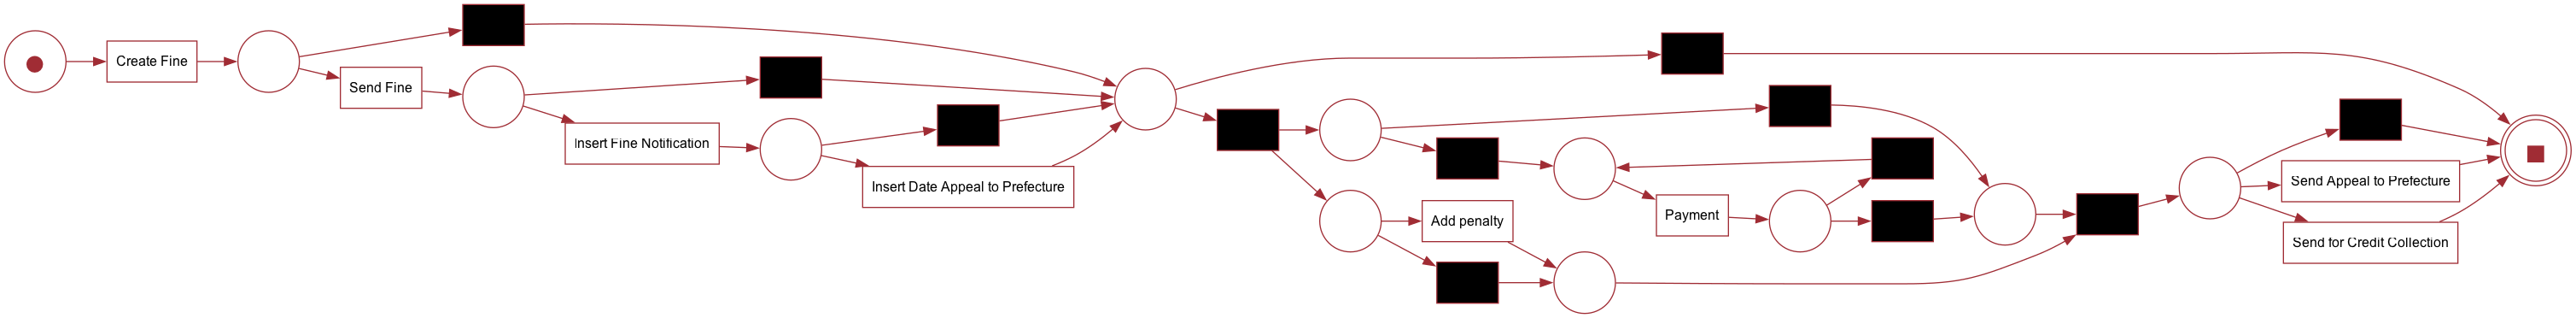
\includegraphics[width=0.95\textwidth]{petri_net.png}
    \caption{Petri net discovered via the Inductive Miner on the top 10 variants.}
    \label{fig:petri_net}
\end{figure}

The Petri net reveals the structural logic of the process. After \textit{Create Fine}, the model shows an exclusive choice: a case either proceeds to \textit{Send Fine} (the standard administrative path) or directly to \textit{Payment} (immediate settlement). Along the standard path, a sequence of \textit{Send Fine} $\rightarrow$ \textit{Insert Fine Notification} $\rightarrow$ \textit{Add penalty} leads to a second exclusive choice between \textit{Payment} and \textit{Send for Credit Collection}. The model also captures a loop on the \textit{Payment} activity, reflecting cases where multiple partial payments are recorded. This structure confirms that the process is fundamentally sequential with two key decision points — one at the beginning (immediate payment vs.\ administrative processing) and one at the end (payment vs.\ escalation).

To evaluate how well this model generalizes to the full event log, Token-Based Replay was performed on a random sample of 2,000 cases drawn from the unfiltered log. The replay yielded:

\begin{itemize}
    \item Percentage of fitting traces: 98.70\%
    \item Average trace fitness: 0.9985
\end{itemize}

The high fitness score confirms that the model discovered from the top 10 variants captures nearly all real-world execution paths, including those not explicitly used during discovery.

\subsection{Conformance Checking: Legal and Operational Compliance}
\label{sub:conformance}

Beyond model fitness, five domain-specific compliance rules were defined based on the Italian Codice della Strada (CdS). Each rule was evaluated programmatically against the full event log. The compliance rate is defined as the fraction of applicable cases that do not violate the rule.

\subsubsection{Rule 1: 90-Day Statutory Deadline (Art.\ 201 CdS)}

The Italian Highway Code requires that notification of an offence is sent within 90 days of the violation. The rule checks whether the time between \textit{Create Fine} and \textit{Send Fine} exceeds 90 days.

\begin{itemize}
    \item Applicable cases: 103,987
    \item Violations: 49,772 (average delay in violation cases: 124 days)
    \item \textbf{Compliance rate: 52.14\%}
\end{itemize}

Nearly half of all applicable cases exceed the statutory deadline. This represents a critical compliance failure that may render affected fines legally contestable.

\subsubsection{Rule 2: 60-Day Penalty Grace Period (Art.\ 202\S1, 203\S3 CdS)}

Citizens must be given at least 60 days after notification before a penalty can be added. The rule checks whether \textit{Add penalty} occurs fewer than 60 days after the notification event.

\begin{itemize}
    \item Applicable cases: 79,860
    \item Violations: 0
    \item \textbf{Compliance rate: 100\%}
\end{itemize}

The administration fully respects the 60-day grace period in all recorded cases.

\subsubsection{Rule 3: Due Process — Appeal Prerequisite (Art.\ 203\S1 CdS)}

An appeal to the Prefecture can only be filed if the offender was previously notified. The rule verifies that \textit{Send Appeal to Prefecture} is preceded by either \textit{Insert Fine Notification} or \textit{Send Fine}.

\begin{itemize}
    \item Applicable cases: 4,141
    \item Violations: 7
    \item \textbf{Compliance rate: 99.83\%}
\end{itemize}

Due process is respected in virtually all appeal cases.

\subsubsection{Rule 4: Duty to Inform (Art.\ 204\S2 CdS)}

When the Prefecture issues a decision on an appeal, the administration must notify the offender of the result. The rule checks whether \textit{Receive Result Appeal from Prefecture} is followed by \textit{Notify Result Appeal to Offender}.

\begin{itemize}
    \item Applicable cases: 761
    \item Violations: 43
    \item \textbf{Compliance rate: 94.35\%}
\end{itemize}

In 43 completed cases, the offender was never informed of the Prefecture's decision — a gap that undermines procedural transparency.

\subsubsection{Rule 5: Payment Accuracy (Art.\ 202\S1, 203\S3 CdS)}

Once the statutory debt is settled through payment, no further payment events should occur. The rule detects cases where additional payments are recorded after the cumulative amount has already met or exceeded the required total.

\begin{itemize}
    \item Applicable cases: 69,715
    \item Violations: 7,522
    \item \textbf{Compliance rate: 89.21\%}
\end{itemize}

Over 7,500 cases contain redundant payment events, suggesting either system errors or manual double-processing.

\subsubsection{Compliance Summary}

\begin{table}[H]
    \centering
    \begin{tabular}{llr}
        \toprule
        \textbf{Rule} & \textbf{Legal Basis} & \textbf{Compliance} \\
        \midrule
        90-Day Statutory Deadline & Art.\ 201 CdS & 52.14\% \\
        60-Day Penalty Grace Period & Art.\ 202\S1, 203\S3 CdS & 100.00\% \\
        Due Process (Appeal Prerequisite) & Art.\ 203\S1 CdS & 99.83\% \\
        Duty to Inform & Art.\ 204\S2 CdS & 94.35\% \\
        Payment Accuracy & Art.\ 202\S1, 203\S3 CdS & 89.21\% \\
        \bottomrule
    \end{tabular}
    \caption{Summary of compliance rule evaluation results}
    \label{tab:compliance_summary}
\end{table}

The most critical finding is the widespread violation of the 90-day notification deadline. The remaining rules show high compliance, with the exception of payment accuracy, where redundant payment events suggest a systematic processing issue rather than intentional misconduct.

\subsection{Bottleneck Analysis}
\label{sub:performance_bottlenecks}

Transition durations — the time elapsed between consecutive activities within a case — were computed to identify operational bottlenecks. Figures~\ref{fig:bottlenecks_mean} and~\ref{fig:bottlenecks_median} show the top five transitions ranked by mean and median duration respectively.

\begin{figure}[H]
    \centering
    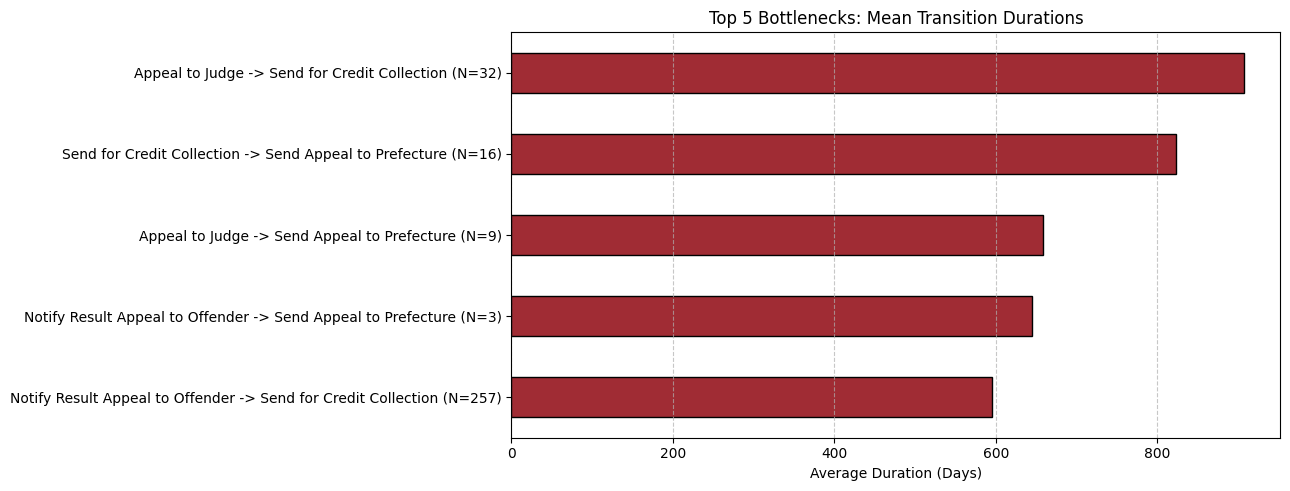
\includegraphics[width=0.9\textwidth]{bottlenecks_mean.png}
    \caption{Top 5 process bottlenecks by mean transition duration (days).}
    \label{fig:bottlenecks_mean}
\end{figure}

\begin{figure}[H]
    \centering
    
\includegraphics[width=0.9\textwidth]{bottlenecks_median.png}
    \caption{Top 5 process bottlenecks by median transition duration (days).}
    \label{fig:bottlenecks_median}
\end{figure}

The mean perspective is dominated by transitions leading to \textit{Send for Credit Collection}, reflecting the long tail of cases that remain unresolved for months or years before escalation. The median perspective highlights a different pattern: the most consistent delay occurs before \textit{Payment}, indicating that the primary bottleneck is driven by citizen response behavior rather than internal administrative processing.

\subsection{Batching Behavior}
\label{sub:batching_analysis}

The Dotted Chart (Figure~\ref{fig:dotted_chart}) reveals a distinctive pattern: events of the same activity type align vertically, meaning dozens of unrelated cases experience the same activity on the same calendar date. This is a clear indicator of batch processing — administrative staff accumulate cases and process them collectively at periodic intervals rather than handling each case immediately upon arrival.

\begin{figure}[H]
    \centering
    
\includegraphics[width=0.95\textwidth]{dotted_chart.png}
    \caption{Dotted Chart showing vertical alignment of events as evidence of batching behavior (sample of 500 cases).}
    \label{fig:dotted_chart}
\end{figure}

The Performance Spectrum (Figure~\ref{fig:performance_spectrum}) provides a complementary view. Steep, near-vertical line segments between \textit{Create Fine}, \textit{Send Fine}, and \textit{Insert Fine Notification} confirm that early administrative steps are executed rapidly and in synchronized batches. In contrast, the transitions toward \textit{Add penalty} and \textit{Payment} show shallow, widely dispersed slopes, reflecting long and variable waiting periods.

\begin{figure}[H]
    \centering
    
\includegraphics[width=0.95\textwidth]{performance_spectrum.png}
    \caption{Performance Spectrum showing processing velocities across major transitions (150 cases).}
    \label{fig:performance_spectrum}
\end{figure}

\subsection{Organizational Perspective}
\label{sub:organizational}

Process mining typically includes an organizational perspective to analyze resource allocation, handovers of work, and individual workloads. In this dataset, however, the \texttt{org:resource} attribute has a fill rate below one percent and contains only placeholder values. The resource identities were anonymized or omitted during the original data extraction by \textcite{deleoni2015}. As a result, organizational mining — such as constructing social network graphs or computing resource-level performance metrics — cannot be performed on this event log. The analysis therefore focuses on the control-flow, time, and compliance perspectives where the data provides sufficient coverage.


\section{Predictive Process Monitoring}
\label{sec:predictive}
% The core Machine Learning section (refer to features.py and train.py).

This section describes the predictive process monitoring pipeline. Two prediction tasks are addressed: outcome classification and remaining time prediction. Following \textcite{teinemaa2019}, the experimental design compares multiple model families across different prefix lengths and feature variants.

\subsection{Experimental Design}

The core experiment evaluates every model in two feature variants:

\begin{itemize}
    \item \textbf{Control-Flow (CF):} Only the sequence of activities in the prefix is used. Features include activity indicators, prefix length, and temporal attributes derived from timestamps.
    \item \textbf{Data-Aware (DA):} In addition to control-flow features, case-level payload attributes are included: \texttt{amount}, \texttt{points}, \texttt{vehicleClass}, and \texttt{article}.
\end{itemize}

Each variant is evaluated at prefix lengths $k \in \{2, 3, 5\}$, representing increasing amounts of observable process history at prediction time. This design allows a systematic comparison of whether data-aware features provide additional predictive value beyond the activity sequence alone.

\subsection{Feature Engineering}
\label{sub:feature_engineering}

Features are constructed from case prefixes following the methodology of \textcite{teinemaa2019}. For each case, only the first $k$ events are used as input — simulating a realistic online prediction scenario where the final outcome is unknown.

For tabular models, the prefix is aggregated into a fixed-length feature vector containing:
\begin{itemize}
    \item Activity indicators: binary flags for each activity observed in the prefix
    \item Temporal features: elapsed time since case start, start year, start month, and start weekday
    \item Prefix length
    \item Payload aggregates (DA variant only): cumulative amount, points, and one-hot encoded vehicle class and article
\end{itemize}

For the LSTM model, the prefix is represented as an ordered integer sequence of activity IDs, padded or truncated to length $k$. In the DA variant, payload features are concatenated to each time step.

Outcome-revealing activities — \textit{Payment} and \textit{Send for Credit Collection} — are excluded from all input features to prevent data leakage. This exclusion is critical: if the model observed \textit{Payment} in the prefix, it could trivially infer the outcome without learning any generalizable pattern. By removing these activities from the input vocabulary, the model is forced to learn from the preceding administrative steps — which is precisely the information available at the point when a prediction would be made in practice.

The resulting feature matrices have modest dimensionality. At $k=2$ in the CF variant, each case is represented by approximately 15 features (activity flags plus temporal attributes). In the DA variant, one-hot encoding of \texttt{article} (grouped into 11 categories) and \texttt{vehicleClass} expands the feature vector to roughly 30 columns. This low dimensionality explains why even simple linear models perform well — the feature space is compact and the signal-to-noise ratio is high.

\subsection{Data Splitting Strategy}

A temporal split ensures that no future information leaks into training. Cases are sorted by their start timestamp and divided into three sets:

\begin{itemize}
    \item Training: 64\% (oldest cases)
    \item Validation: 16\%
    \item Test: 20\% (most recent cases) — 25,321 cases
\end{itemize}

This simulates a deployment scenario where the model is trained on historical data and evaluated on cases that occur later in time.

\subsection{Model Lineup}

Four model families are trained for outcome classification, and four for remaining time regression:

\textbf{Outcome (classification):}
\begin{enumerate}
    \item \textbf{Majority Baseline:} Always predicts the most frequent class.
    \item \textbf{Logistic Regression:} Linear model with standardized features and balanced class weights.
    \item \textbf{Random Forest:} Ensemble of 100 trees with balanced class weights.
    \item \textbf{XGBoost:} Gradient-boosted trees with early stopping on the validation set.
    \item \textbf{LSTM:} Embedding layer → LSTM layer → dropout → linear output, trained with weighted binary cross-entropy.
\end{enumerate}

\textbf{Remaining Time (regression):}
\begin{enumerate}
    \item \textbf{Mean Baseline:} Always predicts the training-set mean duration.
    \item \textbf{Linear Regression}
    \item \textbf{Random Forest Regressor}
    \item \textbf{XGBoost Regressor} (with early stopping)
    \item \textbf{LSTM Regressor:} Same architecture as above with a linear output head.
\end{enumerate}

\subsection{Outcome Classification Results}

Table~\ref{tab:outcome_results} reports the test-set performance for outcome prediction. The primary metrics are AUC-ROC and F1-score for the positive class (credit collection).

\begin{table}[H]
\centering
\begin{tabular}{llccc}
\toprule
\textbf{Model} & \textbf{Variant} & \textbf{$k$} & \textbf{AUC-ROC} & \textbf{F1 (Collection)} \\
\midrule
Majority Baseline & CF & 2 & 0.500 & 0.000 \\
Logistic Regression & CF & 2 & 0.879 & 0.854 \\
Random Forest & CF & 2 & 0.879 & 0.854 \\
XGBoost & CF & 2 & 0.879 & 0.854 \\
LSTM & CF & 5 & 0.888 & 0.855 \\
\midrule
Logistic Regression & DA & 2 & 0.880 & 0.854 \\
Random Forest & DA & 2 & 0.877 & 0.837 \\
XGBoost & DA & 2 & 0.880 & 0.854 \\
LSTM & DA & 5 & 0.889 & 0.854 \\
\bottomrule
\end{tabular}
\caption{Outcome classification results on the temporal test set (selected configurations).}
\label{tab:outcome_results}
\end{table}

Several observations stand out. First, all trained models substantially outperform the majority baseline, confirming that the activity sequence carries strong predictive signal for the outcome. Second, the performance difference between models is remarkably small — Logistic Regression, Random Forest, and XGBoost achieve nearly identical scores at $k=2$. This suggests that the prediction problem is largely linearly separable given the prefix features. Third, longer prefixes provide only marginal improvement: AUC increases from 0.879 at $k=2$ to 0.889 at $k=5$. Fourth, the DA variant does not meaningfully outperform the CF variant, indicating that the activity sequence alone captures most of the predictive information.

\subsection{Remaining Time Prediction Results}

Table~\ref{tab:remaining_results} reports the regression performance measured in Mean Absolute Error (MAE) and Root Mean Squared Error (RMSE), both in days.

\begin{table}[H]
\centering
\begin{tabular}{llccc}
\toprule
\textbf{Model} & \textbf{Variant} & \textbf{$k$} & \textbf{MAE (days)} & \textbf{RMSE (days)} \\
\midrule
Mean Baseline & CF & 2 & 293.0 & 313.1 \\
Linear Regression & CF & 2 & 106.2 & 168.0 \\
Random Forest & CF & 2 & 106.2 & 168.0 \\
XGBoost & CF & 2 & 106.2 & 168.0 \\
LSTM & CF & 5 & 102.3 & 166.2 \\
\midrule
XGBoost & DA & 2 & 99.6 & 162.9 \\
LSTM & DA & 5 & 101.2 & 165.2 \\
\bottomrule
\end{tabular}
\caption{Remaining time prediction results on the temporal test set (selected configurations).}
\label{tab:remaining_results}
\end{table}

All models reduce the MAE from 293 days (mean baseline) to approximately 100–106 days. Unlike outcome prediction, the DA variant provides a modest improvement for remaining time: XGBoost DA achieves an MAE of 99.6 days compared to 106.2 in the CF variant. The payload attribute \texttt{amount} likely contributes information about case complexity that correlates with processing duration.

\subsection{Discussion}

The results reveal that the Road Traffic Fine Management process is highly predictable from minimal prefix information. Even with only two observed activities, models achieve an AUC of 0.88 — a strong result given the early prediction point. The near-identical performance across model families at each prefix length indicates that the underlying signal is well-captured by simple features, and that the process structure leaves limited room for complex models to differentiate themselves.

The convergence of all models at $k=2$ deserves closer examination. An analysis of outcome rates conditioned on the second activity reveals the underlying mechanism: cases whose second activity is \textit{Payment} have a credit collection rate of only 0.1\%, while cases whose second activity is \textit{Send Fine} escalate in 74\% of cases. Since these two activities account for over 99\% of all second events, the second activity alone is nearly sufficient to determine the outcome. This explains why a simple Logistic Regression matches the performance of an LSTM at this prefix length — the decision boundary is essentially a single threshold on one binary feature. At longer prefix lengths ($k=5$), the LSTM gains a marginal advantage because the ordering of subsequent activities (notification, penalty) provides additional sequential context that aggregated tabular features cannot fully represent.

The LSTM provides a slight advantage at longer prefix lengths, where sequential ordering becomes more informative. However, the gain over tabular models is marginal, which is consistent with the observation from Chapter~\ref{sec:eda} that most traces contain only four to five events — limiting the advantage of sequence modeling.

For remaining time prediction, the high residual error (MAE $\approx$ 100 days) reflects the inherent uncertainty of the process: throughput times range from days to years, and much of the variation is driven by external citizen behavior that cannot be predicted from the event log alone. In relative terms, the MAE corresponds to approximately 29\% of the mean throughput time (342 days), representing a substantial reduction in uncertainty compared to the naïve baseline. Nevertheless, this level of precision is best suited for aggregate workload planning — for instance, estimating how many cases will conclude within a given quarter — rather than individual case-level time commitments. For operational decision-making at the case level, the outcome classifier with its prescriptive tier system (Section~\ref{sec:interpretability}) remains the primary tool.


\section{Interpretability and Prescriptive Analytics}
\label{sec:interpretability}
% ==========================================
% SECTION 6: INTERPRETABILITY AND PRESCRIPTIVE ANALYTICS
% ==========================================

While the predictive models from the previous section achieve strong classification performance, understanding \textit{why} a model predicts a particular outcome is equally important — both for building trust in the system and for deriving actionable process improvements. This section applies SHAP-based feature importance analysis to the XGBoost outcome classifier and translates the resulting insights into a prescriptive recommendation system.

\subsection{Feature Importance via SHAP}
\label{sub:shap}

SHAP (SHapley Additive exPlanations) assigns each feature a contribution to the model's prediction for a given instance, grounded in cooperative game theory \parencite{lundberg2017}. Because XGBoost is a tree ensemble, exact Shapley values can be computed efficiently using the TreeExplainer algorithm without approximation.

SHAP summary plots were generated for all combinations of variant (CF, DA) and prefix length ($k \in \{2, 3, 5\}$). Figure~\ref{fig:shap_da_k5} shows the summary for the best-performing configuration (DA, $k=5$).

\begin{figure}[H]
    \centering
    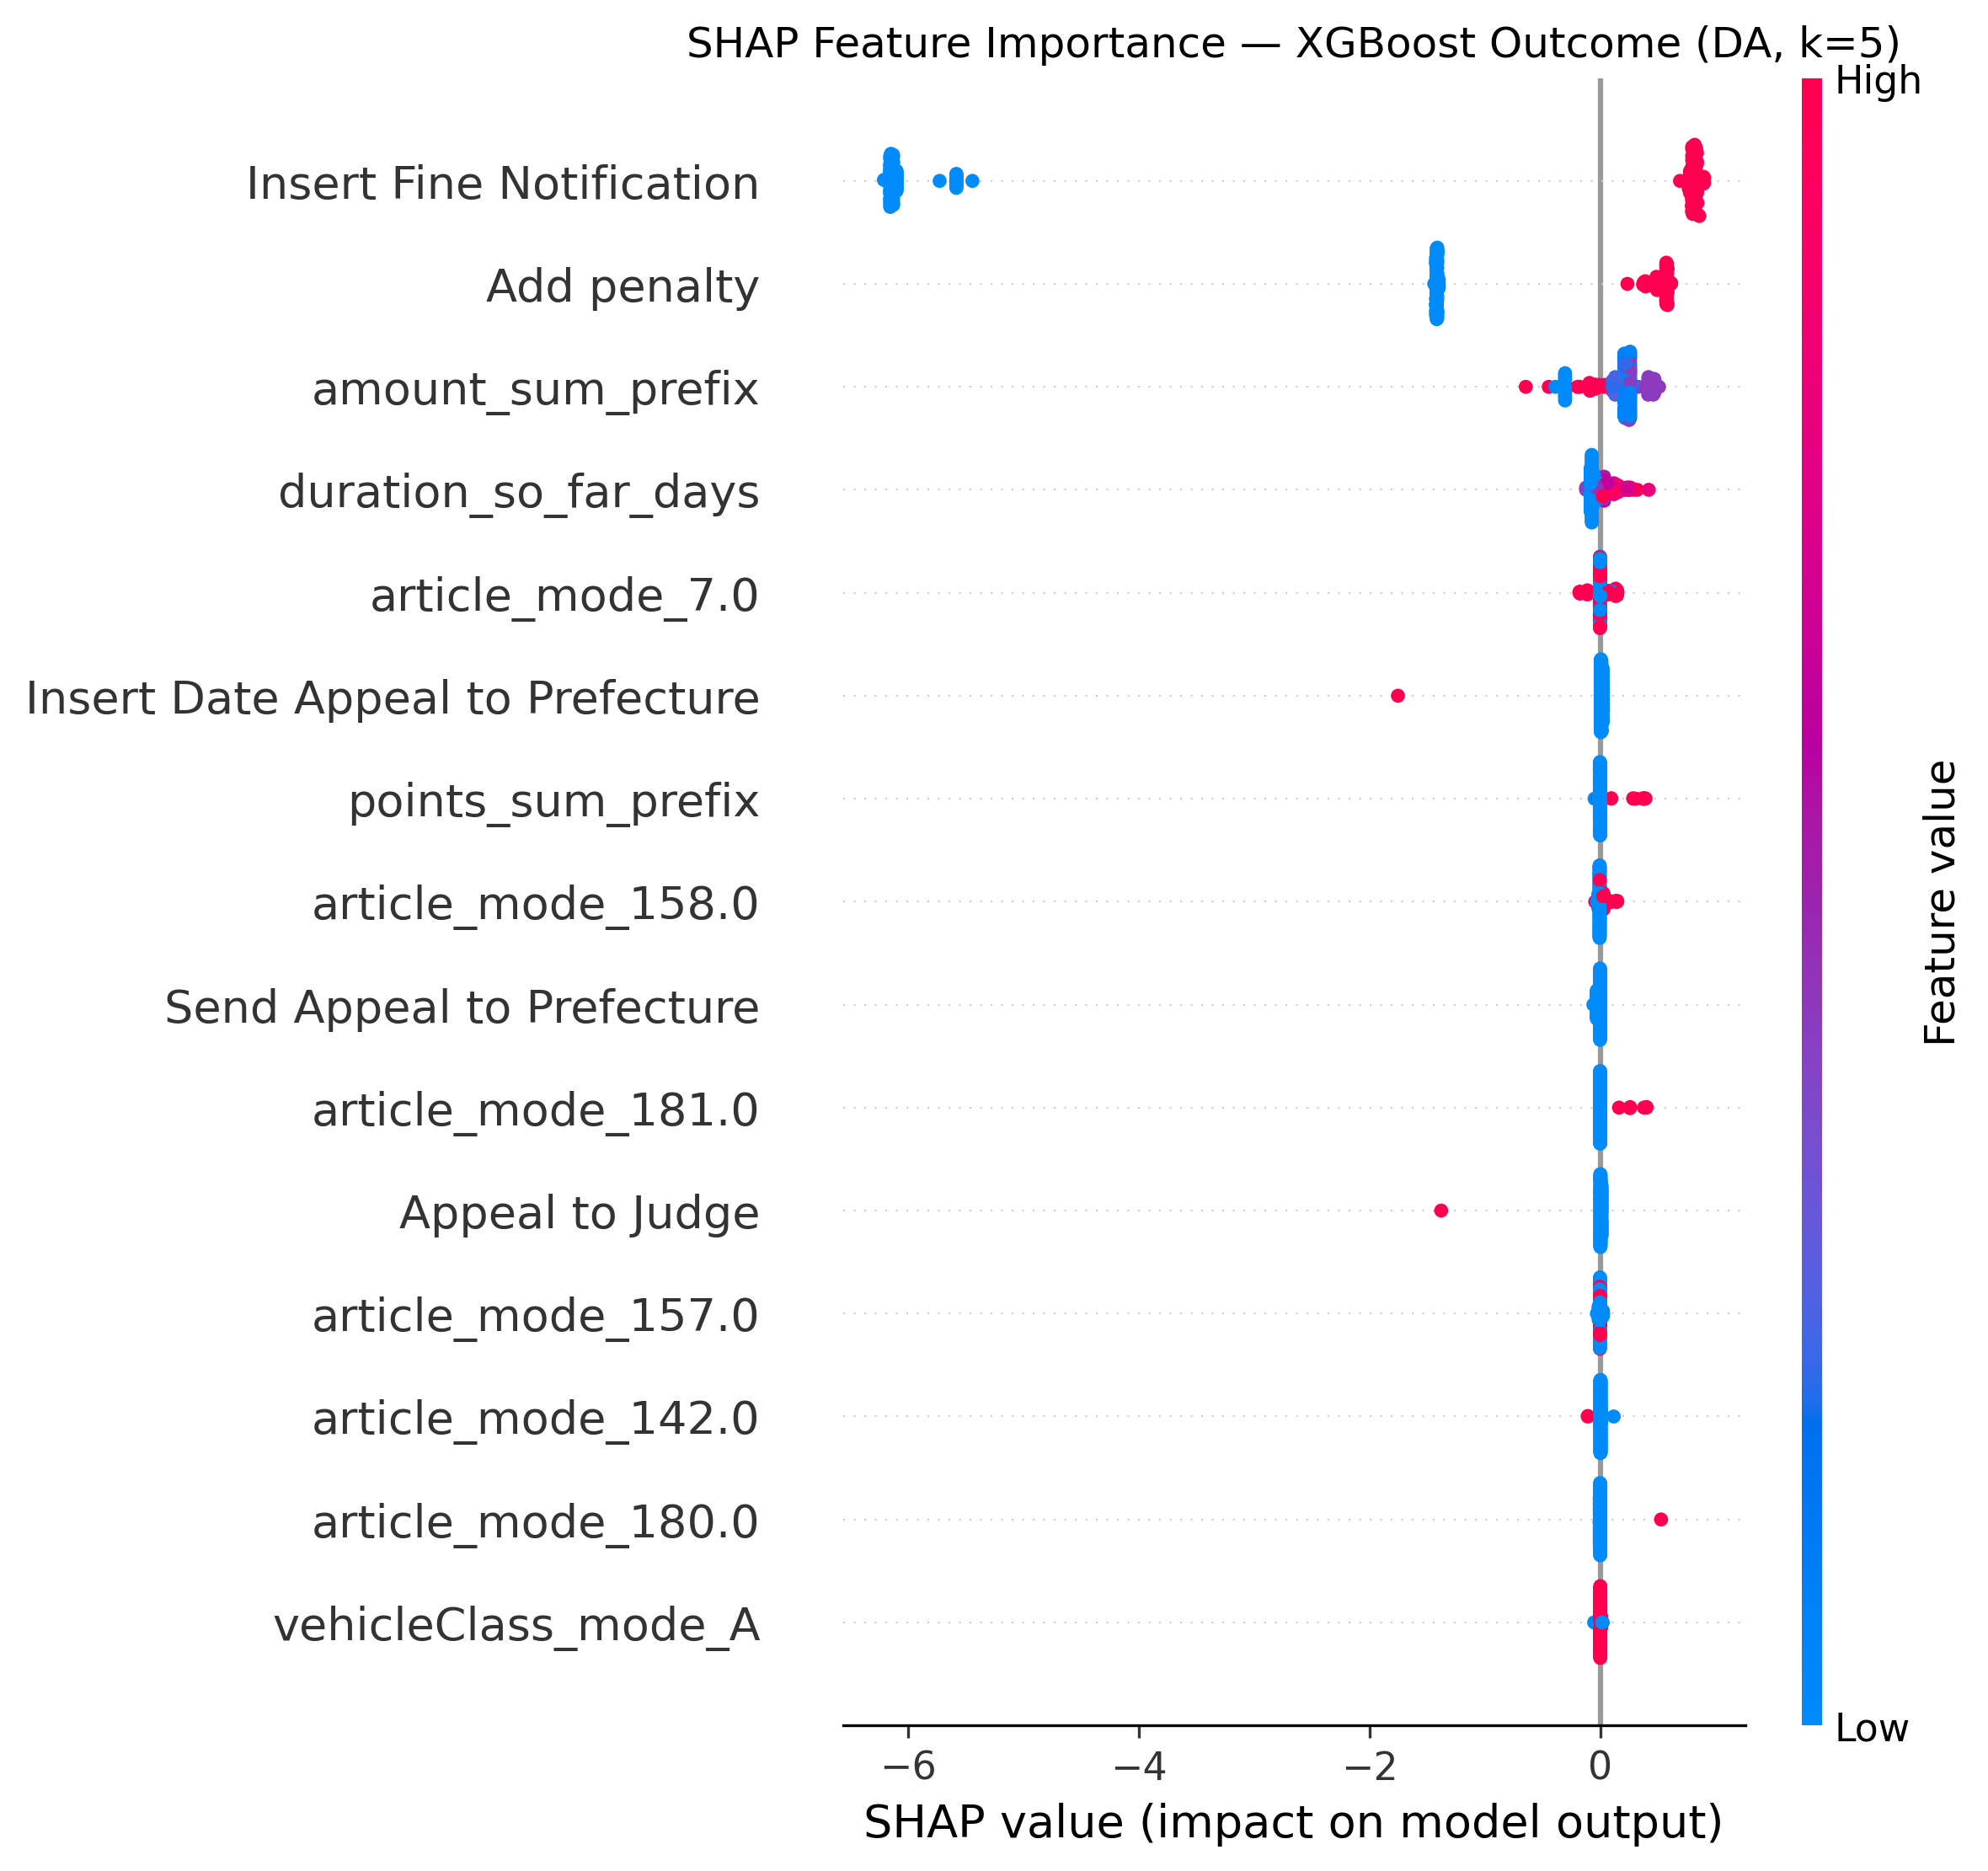
\includegraphics[width=0.9\textwidth]{shap_da_k5.png}
    \caption{SHAP summary plot for XGBoost outcome classifier (DA variant, $k=5$). Each dot represents one test case; the horizontal position shows the feature's contribution to the prediction.}
    \label{fig:shap_da_k5}
\end{figure}

The SHAP analysis reveals the following key drivers of credit collection risk:

\begin{itemize}
    \item \textbf{Activity indicators:} The presence of \textit{Add penalty} and \textit{Insert Fine Notification} in the prefix strongly pushes predictions toward class~1 (credit collection). Conversely, an early \textit{Payment} event dominates predictions toward class~0.
    \item \textbf{Elapsed time:} Longer time since case start correlates with higher predicted risk — cases that remain unresolved for extended periods are more likely to escalate.
    \item \textbf{Fine amount:} Higher amounts show a moderate positive association with credit collection risk in the DA variant.
\end{itemize}

Figure~\ref{fig:shap_cf_k5} shows the SHAP summary for the CF variant at the same prefix length for comparison.

\begin{figure}[H]
    \centering
    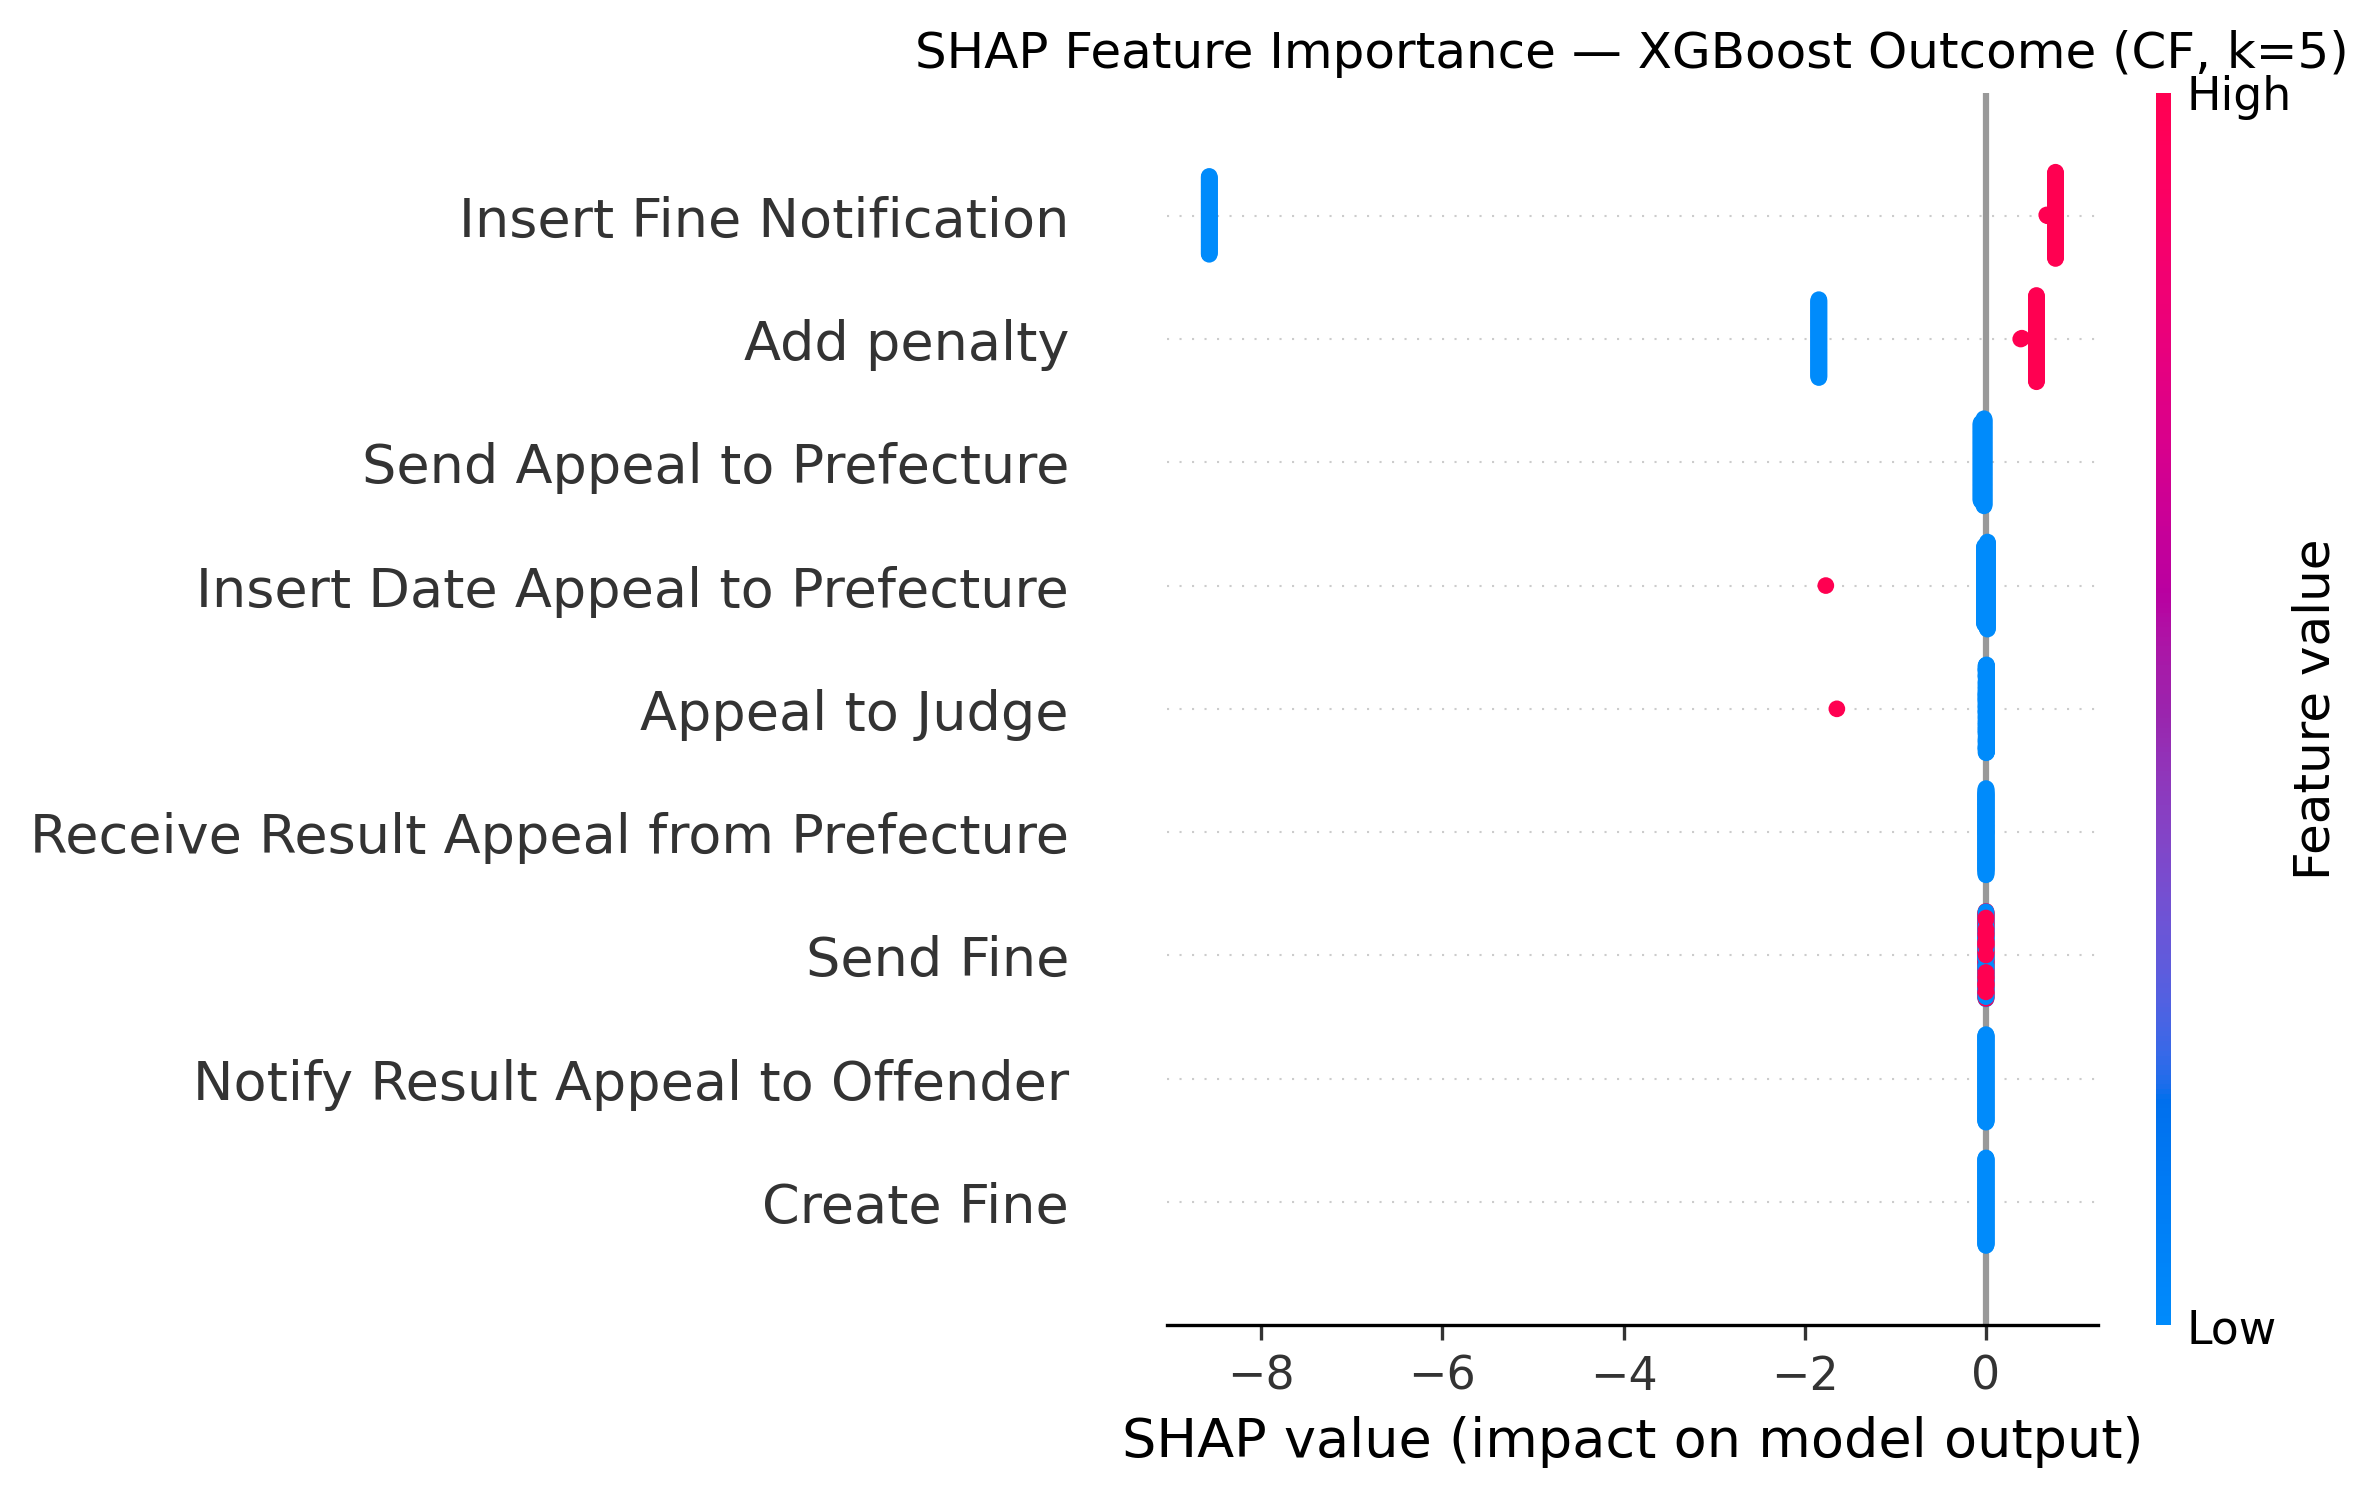
\includegraphics[width=0.9\textwidth]{shap_cf_k5.png}
    \caption{SHAP summary plot for XGBoost outcome classifier (CF variant, $k=5$). Without payload attributes, the model relies entirely on activity indicators and temporal features.}
    \label{fig:shap_cf_k5}
\end{figure}

Comparing the two variants reveals why data-aware features provide minimal improvement for outcome prediction. In the CF plot, the activity indicators \textit{Add penalty} and \textit{Insert Fine Notification} already dominate the prediction — their presence in the prefix is a near-deterministic signal for credit collection. When payload attributes such as \texttt{amount} and \texttt{points} are added in the DA variant, they appear in the SHAP ranking but with substantially smaller effect sizes. The activity sequence has already captured the escalation trajectory; the numeric attributes merely provide redundant confirmation.

This finding has a practical implication: for outcome prediction, a deployment could rely on the simpler CF model without collecting or maintaining payload data, reducing implementation complexity while sacrificing negligible predictive performance.

\subsection{Prescriptive Process Monitoring}
\label{sub:prescriptive}

Prescriptive analytics extends prediction into actionable recommendations. Rather than merely forecasting which cases will escalate, the system recommends specific interventions based on the predicted probability of credit collection.

\subsubsection{Policy Design}

A threshold-based action policy assigns each active case to a risk tier based on the XGBoost model's predicted probability $p$ of credit collection:

\begin{itemize}
    \item $p \geq 0.75$ — \textbf{RED}: Immediate escalation. Proactively offer a payment plan to prevent costly debt collection.
    \item $0.50 \leq p < 0.75$ — \textbf{YELLOW}: Send a manual reminder or initiate proactive contact.
    \item $p < 0.50$ — \textbf{GREEN}: No intervention required. The case is likely to resolve through normal payment.
\end{itemize}

The thresholds are motivated by a cost-benefit analysis. A prevented credit collection saves an estimated 120 EUR in administrative and agency costs, while proactive outreach costs approximately 15 EUR and a reminder costs 5 EUR. The expected net gain of an intervention is:
\begin{equation*}
    \text{Expected Gain} = p \cdot \text{Benefit}_{\text{prevented}} - \text{Cost}_{\text{action}}
\end{equation*}

At $p = 0.75$, immediate escalation yields an expected gain of approximately 75 EUR per case — well above the intervention cost. The cost parameters used here are illustrative assumptions; in a production deployment, they would need to be calibrated from historical intervention data and actual recovery rates.

\subsubsection{Results}

The policy was applied to the full temporal test set (24,436 cases) using the XGBoost DA model at $k=5$:

\begin{itemize}
    \item \textbf{RED} (escalate): 12,929 cases (52.9\%)
    \item \textbf{YELLOW} (reminder): 362 cases (1.5\%)
    \item \textbf{GREEN} (no action): 11,145 cases (45.6\%)
\end{itemize}

\begin{figure}[H]
    \centering
    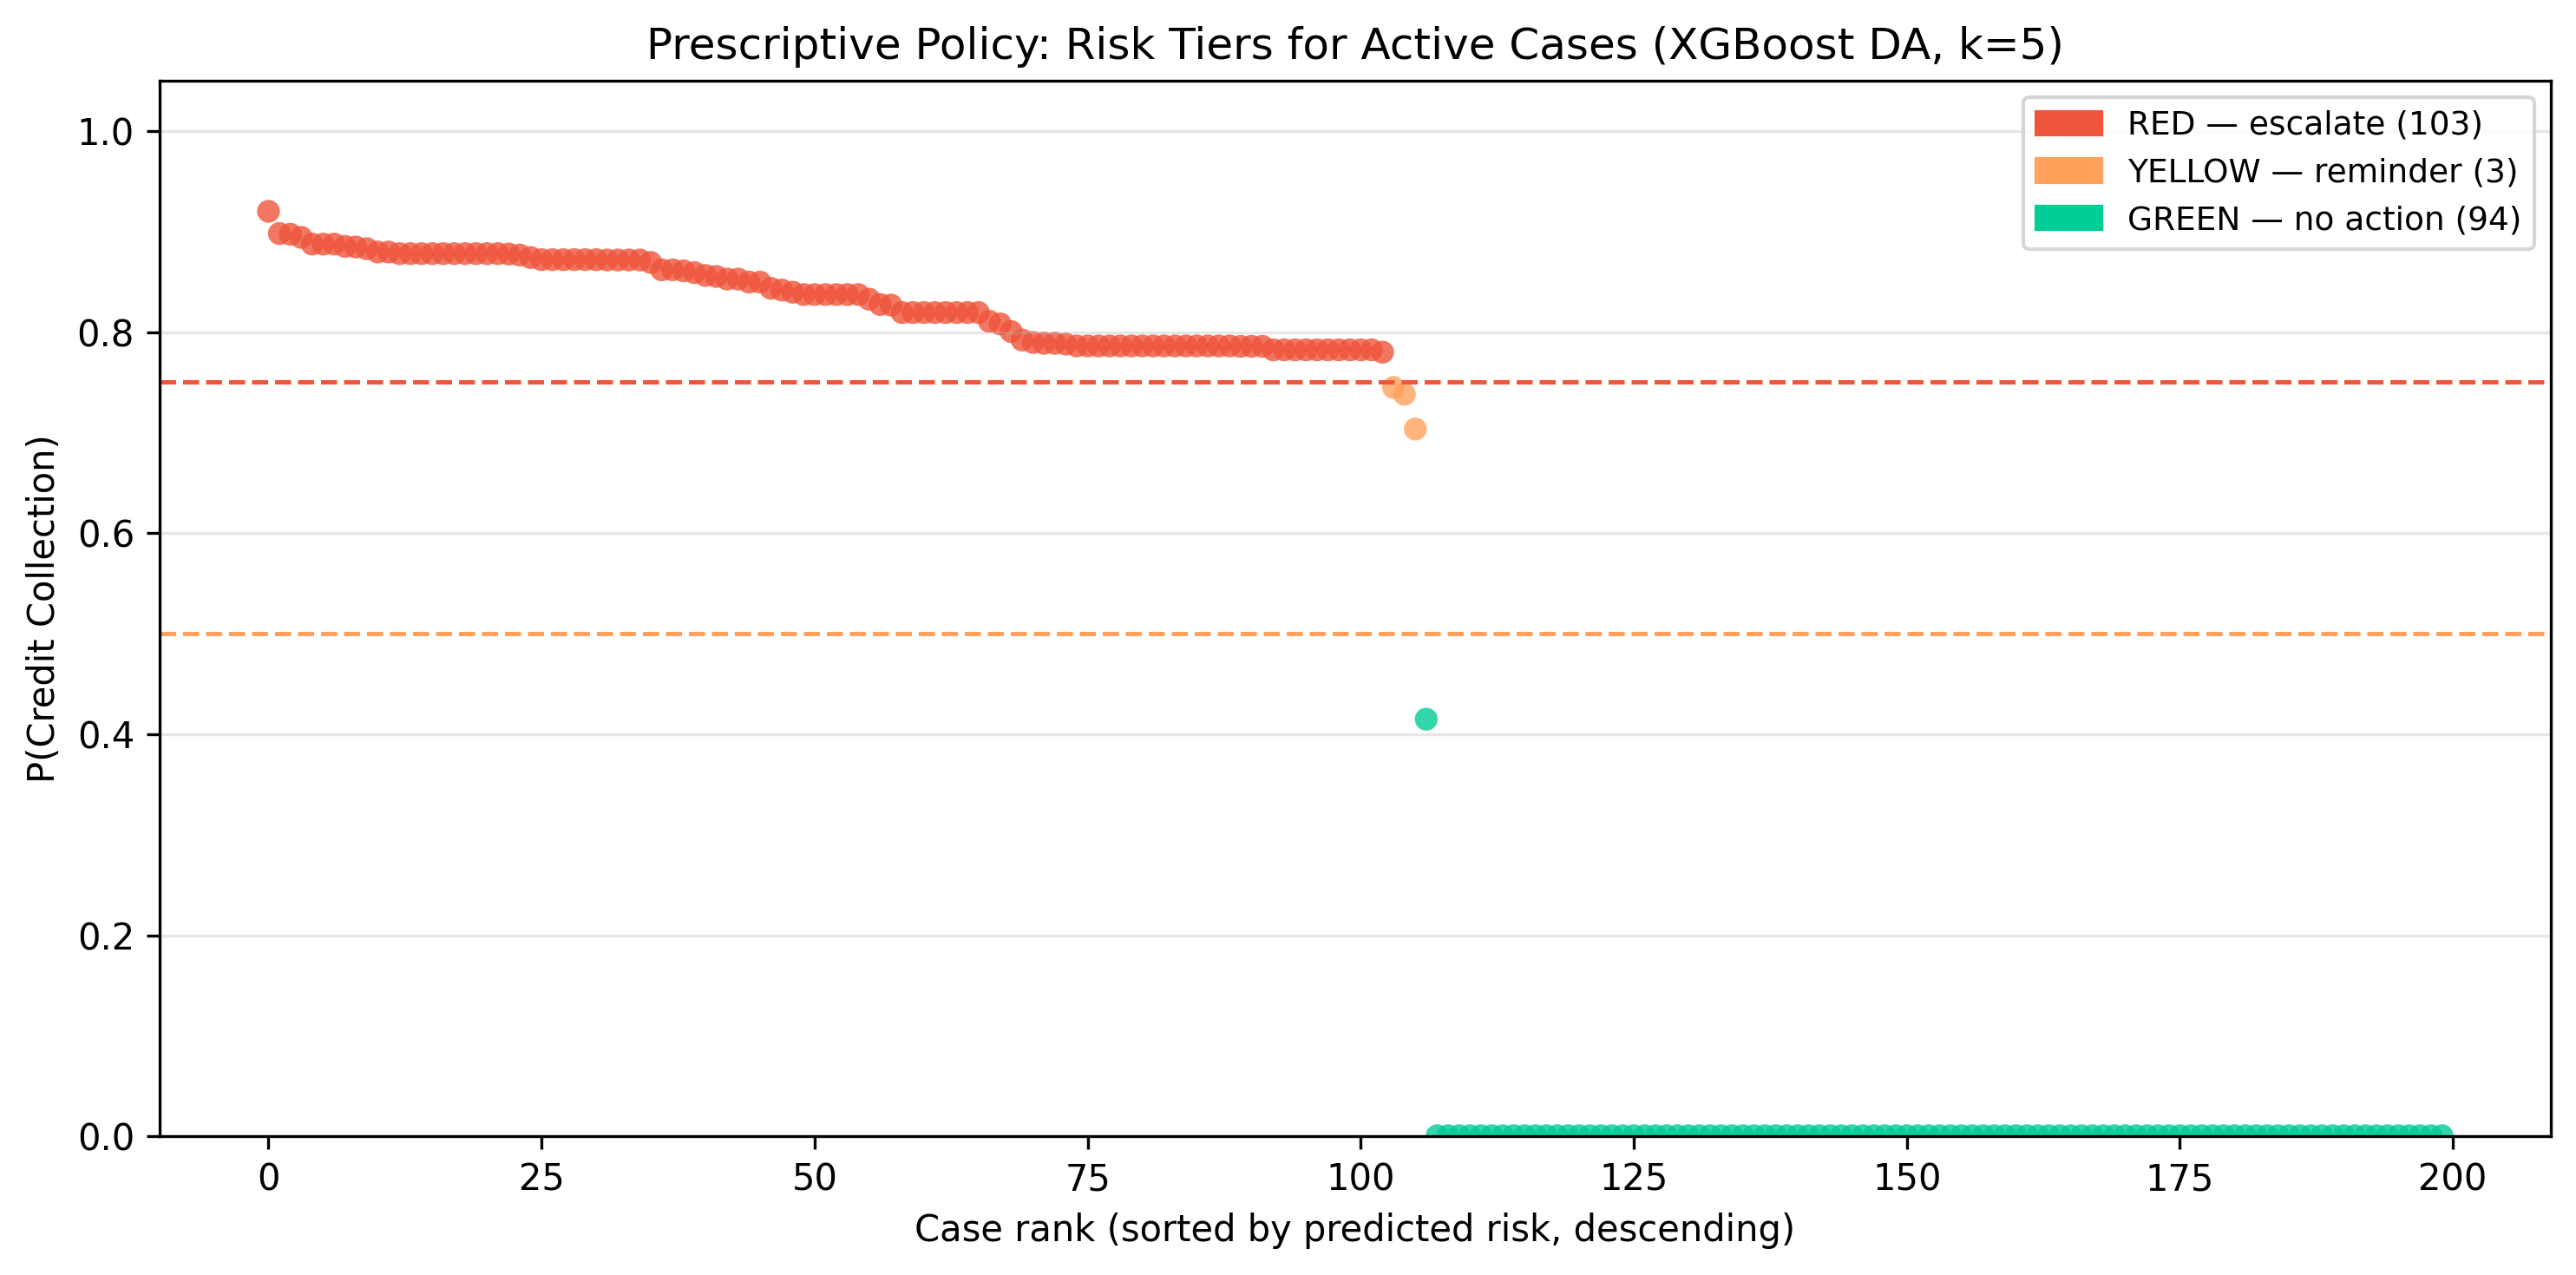
\includegraphics[width=0.85\textwidth]{prescriptive_risk_tiers.png}
    \caption{Distribution of predicted risk scores across the three policy tiers.}
    \label{fig:prescriptive_tiers}
\end{figure}

The bimodal distribution — most cases cluster near either high or low predicted risk — reflects the process structure observed in the variant analysis: cases tend to follow either the payment path or the collection path with relatively few ambiguous intermediate cases. The narrow YELLOW band confirms that the model produces well-separated predictions, making the threshold-based policy straightforward to apply in practice.


\section{Generative AI for Synthetic Event Logs}
\label{sec:generative}
% ==========================================
% SECTION 7: GENERATIVE AI
% ==========================================

This section describes the generation of a synthetic event log using a first-order Markov chain learned from the real process data. Synthetic logs are useful for data augmentation, privacy-preserving data sharing, and stress-testing process models without exposing sensitive operational records.

\subsection{Markov Chain Approach}
\label{sub:markov_chain}

A first-order Markov model was learned from the completed cases in the event log. For each activity, the model records the empirical probability distribution over possible successor activities (including a terminal state). Trace generation starts at \textit{Create Fine} and samples successor activities according to the learned transition probabilities until a terminal state is reached or a maximum trace length of 20 events is exceeded.

This approach is simple to implement and computationally inexpensive. However, it captures only immediate transitions and cannot reproduce long-range dependencies — for instance, repeated payment cycles or sequences that depend on events more than one step in the past. Higher-order Markov models or neural sequence generators would improve structural fidelity but are beyond the scope of this bonus task.

\subsection{Quality Assessment}
\label{sub:gen_quality}

The synthetic log was evaluated against the real event log on three metrics:

\textbf{Activity frequency distribution.} The Jensen-Shannon divergence between the real and synthetic activity distributions is 0.000225 (on a scale where 0 indicates identical distributions and 0.69 represents maximum divergence). Table~\ref{tab:gen_activity} shows that individual activity frequencies match within one percentage point.

\begin{table}[H]
\centering
\begin{tabular}{lrr}
\toprule
\textbf{Activity} & \textbf{Real (\%)} & \textbf{Synthetic (\%)} \\
\midrule
Create Fine & 25.31 & 25.54 \\
Send Fine & 16.04 & 15.88 \\
Insert Fine Notification & 15.32 & 15.19 \\
Add penalty & 15.32 & 14.86 \\
Payment & 15.51 & 16.57 \\
Send for Credit Collection & 11.80 & 11.16 \\
\bottomrule
\end{tabular}
\caption{Activity frequency comparison between real and synthetic event logs (top 6 activities).}
\label{tab:gen_activity}
\end{table}

\textbf{Trace length distribution.} The real log has a mean trace length of 3.95 events (std: 1.58), while the synthetic log produces a mean of 3.92 (std: 1.49). Figure~\ref{fig:gen_trace_length} shows that the two distributions align closely.

\begin{figure}[H]
    \centering
    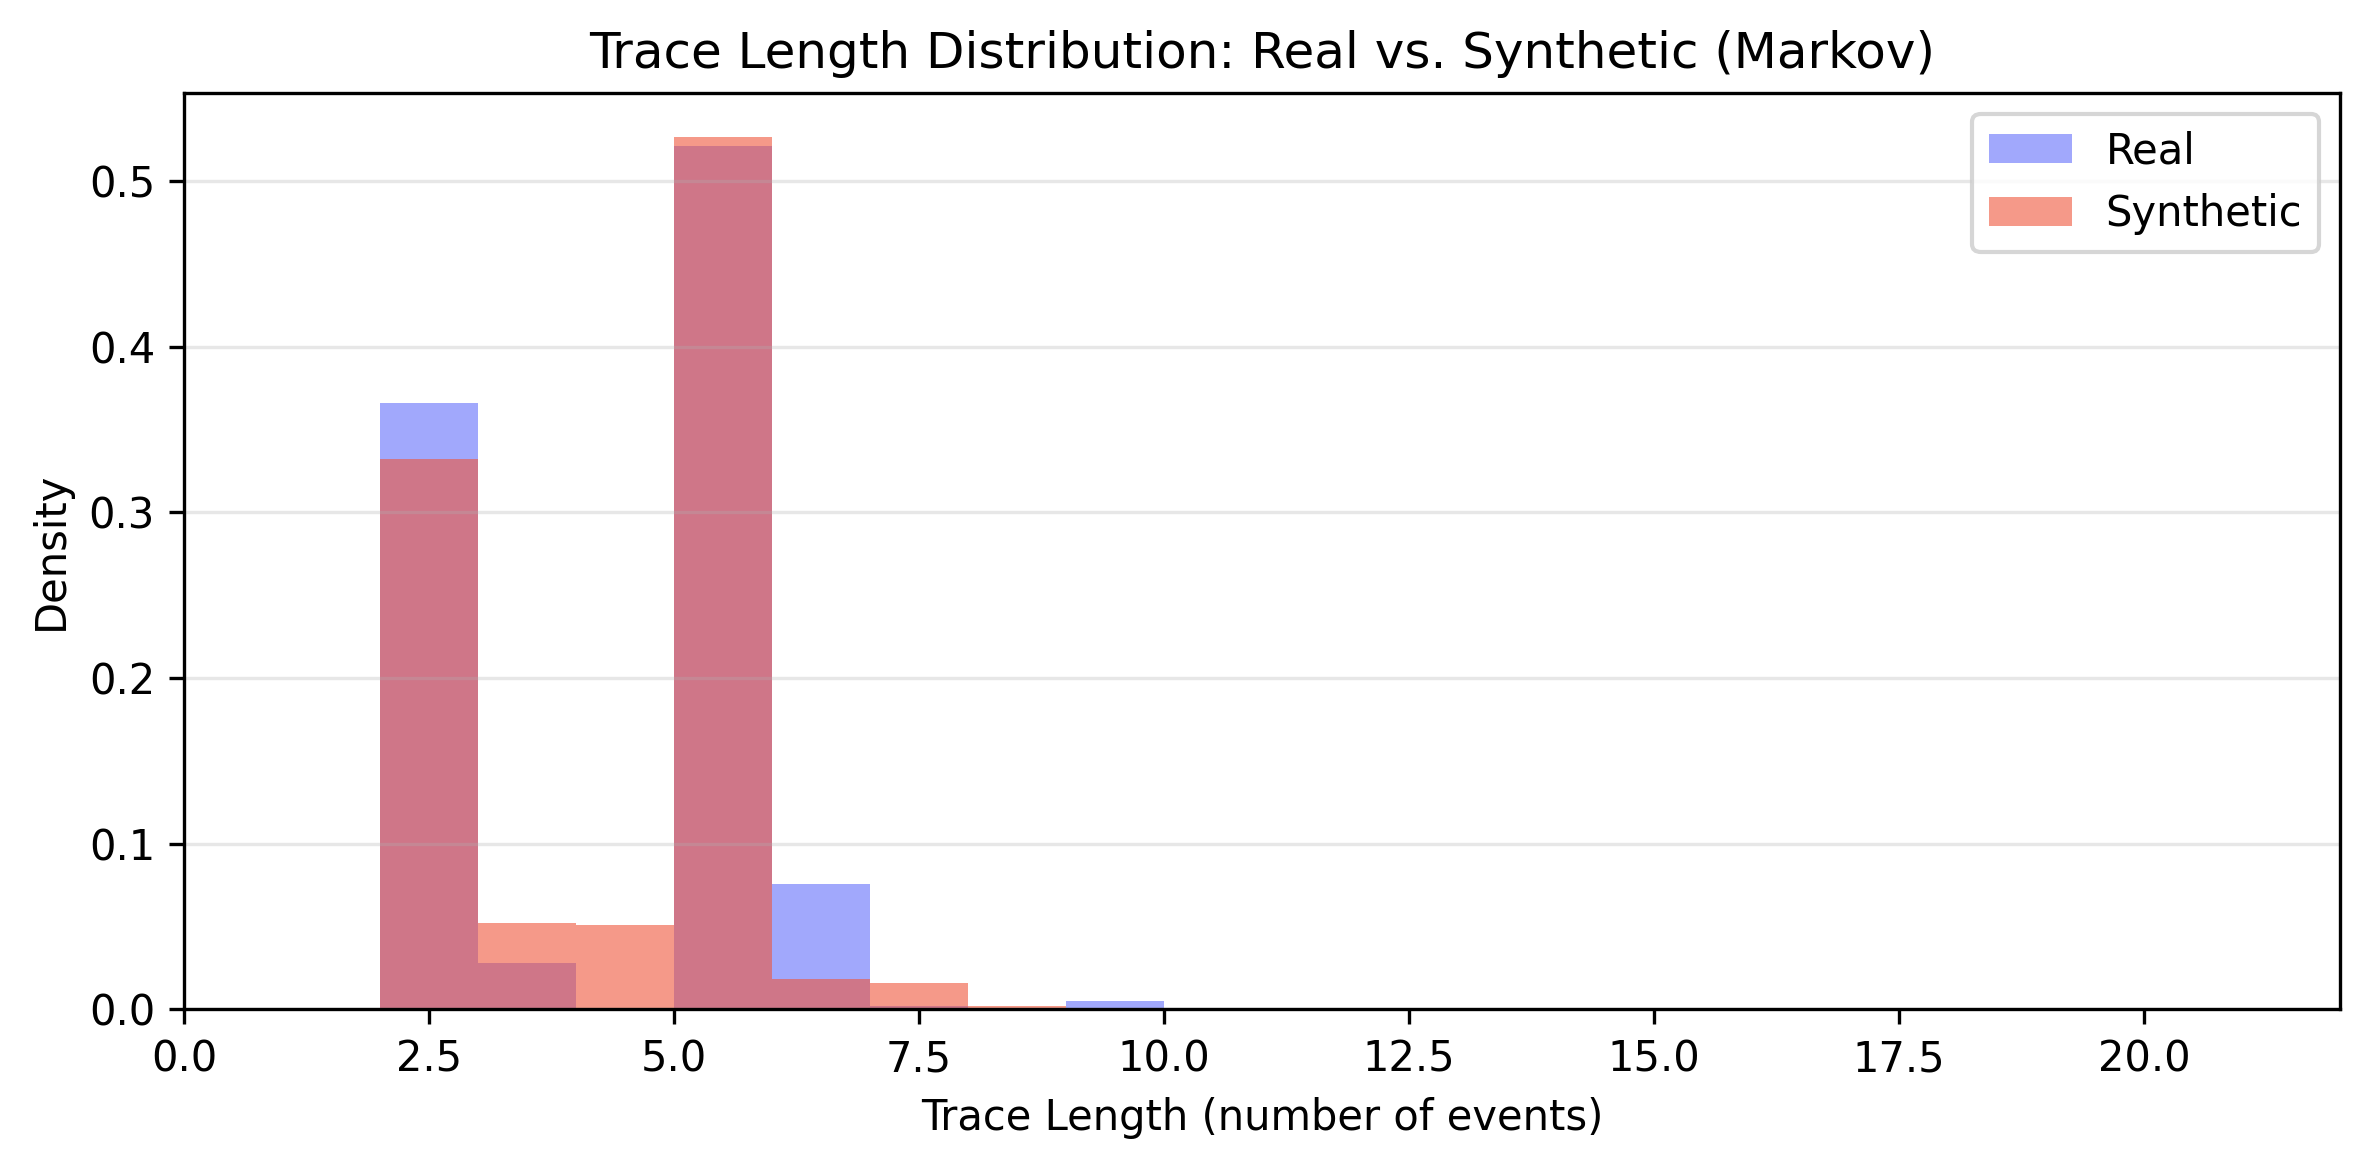
\includegraphics[width=0.8\textwidth]{generative_trace_length_comparison.png}
    \caption{Trace length distribution: real vs.\ synthetic event log.}
    \label{fig:gen_trace_length}
\end{figure}

\textbf{Directly-follows coverage.} The synthetic log reproduces 28 of the 67 directly-follows pairs observed in the real log (41.8\% coverage). This is the primary limitation of the first-order model: rare transitions — particularly those involving appeal activities — are underrepresented because the Markov chain favors high-probability paths. The dominant process variants are reproduced faithfully, but the tail of infrequent behavior is not fully captured.

\subsection{Limitations and Future Work}

The Markov chain approach succeeds at replicating the aggregate statistical properties of the event log (activity frequencies, trace lengths) but falls short on structural diversity. A more capable synthetic log generator would require at least a second-order model or a neural approach to capture the full range of process behavior. Additionally, the current implementation does not generate realistic timestamps — extending the model with inter-event time distributions would be a natural next step.


\section{Prototypical Deployment}
\label{sec:deployment}
% ==========================================
% SECTION 8: PROTOTYPICAL DEPLOYMENT
% ==========================================

To make the analytical results accessible beyond the Python pipeline, a prototypical web application was developed using Streamlit. The dashboard allows administrative decision-makers to explore process data, evaluate model performance, and interact with the predictive system without requiring programming knowledge.

\subsection{Architecture}
\label{sub:architecture}

The application is built as a multi-tab Streamlit dashboard. The main entry script (\texttt{app/app.py}) routes to six isolated tab modules stored in \texttt{app/tabs/}, maintaining a clear separation of concerns. Heavy data objects — dataframes, trained models, and precomputed reports — are loaded once at startup using Streamlit's \texttt{@st.cache\_data} and \texttt{@st.cache\_resource} decorators to ensure responsive interaction despite the large event log size.

All visualizations use Plotly Express for interactivity: users can zoom, hover for details, and filter dynamically without reloading the page.

\subsection{Dashboard Tabs}
\label{sub:functionalities}

The interface is organized into six tabs that mirror the analytical pipeline:

\paragraph{Tab 1: Data Explorer.}
Displays high-level KPIs (total events, cases, activities), the activity frequency distribution, fine amount histogram, case length statistics, and a monthly workload timeline.

\paragraph{Tab 2: Process Discovery.}
Renders the Petri net as an interactive SVG via Streamlit's \texttt{st.graphviz\_chart()} by parsing the saved DOT file directly. Includes the top process variants, bottleneck charts (mean and median transition durations), and the Performance Spectrum and Dotted Chart as interactive scatter plots for visual batching analysis.

\paragraph{Tab 3: Model Performance.}
Provides a tabular and visual comparison of all trained models across prefix lengths and feature variants. Displays AUC-ROC, F1-score, precision, and recall for outcome classification, as well as MAE and RMSE for remaining time prediction.

\paragraph{Tab 4: Predictive System.}
Functions as a live prediction tool. The user selects a prefix length and feature variant, then inputs case attributes through sliders and checkboxes. The embedded XGBoost classifier outputs a probability score and assigns the case to a risk tier (GREEN / YELLOW / RED) with a corresponding action recommendation. A SHAP waterfall plot provides local explainability for each individual prediction.

\paragraph{Tab 5: Conformance Checking.}
Visualizes the five compliance rule results from Section~\ref{sub:conformance}, displaying compliance rates and violation counts in an interactive bar chart format.

\paragraph{Tab 6: Generative AI.}
Shows the synthetic log quality metrics (JSD, trace length comparison, directly-follows coverage) and allows users to download the generated synthetic event log as a CSV file.

\subsection{Deployment Considerations}
\label{sub:deployment_notes}

The application runs locally via \texttt{streamlit run app/app.py} and requires the trained models and feature files to be present in \texttt{outputs/} and \texttt{data/features/}. For a production deployment, the application could be containerized and served behind a reverse proxy. However, since this is a university prototype, no authentication, logging, or horizontal scaling was implemented.


\section{Conclusion and Future Work}
\label{sec:conclusion}
% ==========================================
% SECTION 9: CONCLUSION AND FUTURE WORK
% ==========================================

\subsection{Summary of Findings}
\label{sub:summary}

This project applied an end-to-end process analytics pipeline to the Road Traffic Fine Management event log, combining process discovery, conformance checking, predictive monitoring, and prescriptive recommendations. The research questions posed in the introduction can now be answered:

\textbf{RQ1 (Process Discovery):} The process is structurally simple — two variants account for over 68\% of all completed cases. The Petri net discovered from the top 10 variants achieves 98.7\% trace fitness on the full log. The primary bottleneck lies in the transition toward credit collection, with mean delays exceeding several hundred days.

\textbf{RQ2 (Operational Behavior):} Batching behavior is clearly visible in the Dotted Chart: administrative activities such as \textit{Send Fine} and \textit{Add penalty} are executed in bulk on specific calendar dates rather than continuously. The Performance Spectrum confirms that early process steps are executed rapidly in synchronized batches, while later steps exhibit long, variable waiting periods driven by citizen response behavior.

\textbf{RQ3 (Predictive Monitoring):} Outcome prediction achieves an AUC-ROC of 0.889 using an LSTM at prefix length $k=5$, though even a simple Logistic Regression at $k=2$ reaches 0.879. The activity sequence alone (CF variant) captures nearly all predictive signal — data-aware features provide only marginal improvement. Remaining time prediction reduces the baseline MAE from 293 to approximately 100 days.

\textbf{RQ4 (Prescriptive Analytics):} SHAP analysis identifies the presence of penalty-related activities and elapsed time as the dominant risk drivers. A threshold-based policy translates predicted probabilities into tiered action recommendations (escalate, remind, or monitor), enabling proactive case management.

\subsection{Limitations}
\label{sub:limitations}

Several limitations constrain the generalizability of this work:

\begin{itemize}
    \item \textbf{Missing resource data:} The event log lacks a usable \texttt{org:resource} attribute, preventing any organizational perspective analysis.
    \item \textbf{Date-only timestamps:} All timestamps are recorded at day granularity, making intra-day performance analysis impossible.
    \item \textbf{Historical data:} The log covers 2000–2013. Process behavior, legal frameworks, and administrative systems may have changed since then.
    \item \textbf{Cost parameters:} The prescriptive recommendations rely on illustrative cost assumptions that would require calibration with real operational data.
    \item \textbf{Model saturation:} The near-identical performance across model families suggests that the prediction problem is largely solved by simple features. More complex architectures do not yield meaningful improvements on this dataset.
\end{itemize}

\subsection{Future Work}
\label{sub:future_work}

Possible extensions include: applying Transformer-based sequence models to evaluate whether attention mechanisms capture long-range dependencies better than LSTMs; implementing online process mining for real-time case monitoring as events arrive; integrating actual cost data from the administration to calibrate the prescriptive policy; and extending the approach to other administrative domains where similar fine-to-collection escalation processes exist.

% ==========================================
% BIBLIOGRAPHY
% ==========================================
\clearpage
\printbibliography

\end{document}